% BEGIN PREAMBEL
\documentclass[9pt, xcolor=dvipsnames, table]{beamer}
\usepackage[british]{babel}
\usepackage{xcolor}
\usepackage{multimedia}
\usepackage{amsmath,amsfonts,amssymb}
\usepackage{upgreek}
\usepackage[version=3]{mhchem}
\usepackage{lmodern}
\usepackage{graphicx}
\usepackage{multicol}
\usepackage{color}
\usepackage{tabularx}
\usepackage{pgfpages}
\usepackage{fontawesome}
\usepackage{wrapfig}
\usepackage{siunitx}
\usepackage{fontspec}
\usepackage{tikz}
\usepackage{textpos}
\usepackage{booktabs}
\usepackage{caption}
\usepackage{subcaption}
\usepackage{wasysym}
\usepackage{animate}
\usepackage{ETHlogo}
\usepackage{xparse}
\newfontfamily\ubuntu{Ubuntu}

\newcommand{\li}{\left|}
\newcommand{\re}{\right|}
\newcommand{\const}{\text{const.}}
\newcommand{\z}{\text}
\newcommand{\terminal}[1]{\colorbox{black}{\textcolor{white}{{\fontfamily{phv}\selectfont \scriptsize{#1}}}}}
\newcommand{\plugin}[1]{\textit{\flq#1\frq}}
\newcommand{\ra}{$\rightarrow$ }
\newcommand{\ar}{\autoref}
\newcommand{\good}[1]{{\textcolor{ForestGreen}{\textbf{#1}}}}
\newcommand{\bad}[1]{\textcolor{RedOrange}{\textbf{#1}}}
\newcommand{\dead}[1]{\textcolor{NavyBlue}{\textbf{#1}}}
\newcommand{\cmark}{\good{\ding{51}}}
\newcommand{\xmark}{\bad{\ding{55}}}
\newcommand{\itemfill}{\setlength{\itemsep}{\fill}}
\newcommand{\orderof}[1]{$\mathcal{O}\left(#1\right)$}
\newcommand{\code}[1]{{\footnotesize\dejavu #1}}
\newcommand{\var}[1]{\textcolor{JungleGreen}{#1}}
\newcommand{\meth}[1]{\textcolor{RedOrange}{#1}}
\newcommand{\incl}[1]{\textcolor{YellowGreen!70!RawSienna!100}{#1}}
\newcommand{\str}[1]{\textcolor{MidnightBlue!60!black!100}{#1}}
\newcommand{\tline}[1]{\noalign{\hrule height #1pt}}
\newcommand{\fatwhite}[1]{\multicolumn{1}{c}{\textcolor{white}{\textbf{#1}}}}
\renewcommand{\deg}{$^{\circ}$}
\newcommand{\fpath}[1]{\textbf{\path{#1}}}
\renewcommand\tabularxcolumn[1]{m{#1}}
\newcommand{\alternatecolors}{\rowcolors{2}{gray!5}{gray!15}}
\newcommand{\missfig}[1][.5]{\begin{center} \missingfigure[figheight=#1\textheight,figwidth=#1\textheight, figcolor=white]{}\end{center}}
\newcommand{\caplab}[2]{\ifthenelse{\equal{#1}{nocap}}{}{\caption{#1}}\ifthenelse{\equal{#2}{nolab}}{}{\label{#2}}}
\newcommand{\pic}[3]{\ifthenelse{\equal{#1}{r}}{\includegraphics[width={#2\textheight}, angle=-90]{#3}}{\includegraphics[height={#2\textheight}]{#3}}}
%SUBFIG
\DeclareDocumentCommand{\subfig}{O{.45} O{0} m O{l} m O{nocap} O{nolab}}{\begin{subfigure}{#1\linewidth}\vspace*{#2\textheight}\centering\fig[#4]{#3}{#5}[#6][#7]\end{subfigure}}
%SUBFIGS
\DeclareDocumentCommand{\subfigs}{O{fig} m m O{nocap} O{nolab}}{\begin{figure}[ht!]\centering\ifthenelse{\equal{#1}{fig}}{}{#1\hspace*{.05\linewidth}}#2\hspace*{.05\linewidth}#3\caplab{#4}{#5}\end{figure}}
%FIG
\DeclareDocumentCommand{\fig}{O{n} m m O{nocap} O{nolab}}{\begin{figure}[h!]\centering\pic{#1}{#2}{#3}\caplab{#4}{#5}\end{figure}}
% WRAPFIG
\DeclareDocumentCommand{\wrapfig}{O{l} m m O{nocap} O{nolab}}{
	\begin{wrapfigure}{#1}{#2\linewidth}\includegraphics[width={.95\linewidth}]{#3}\caplab{#4}{#5}\end{wrapfigure}}
\DeclareSIUnit\mhzcm{\mega\hertz\per\centi\meter^2}
\DeclareSIUnit\khzcm{\kilo\hertz\per\centi\meter^2}
\DeclareSIUnit\ncm{n\per\centi\meter^2}

\usetheme{Boadilla}
\graphicspath{ {pics/} }
\makeatletter
\def\input@path{ {sections/} }
\makeatother
\usecolortheme[named=darkgray]{structure}
\useoutertheme{shadow}
\beamertemplatenavigationsymbolsempty
\makeindex
\author[M. Reichmann]{Michael Reichmann}
\institute[\textbf{\textit{ETH}}\scalebox{.6}{\textit{Z\"{u}rich}}]{Swiss Federal Institute of Technology Zurich}
\AtBeginSection{{\setbeamertemplate{headline}{}\frame[noframenumbering]{\sectionpage}}}
\sisetup{detect-weight=true, detect-family=true, range-units=single, range-phrase=$\ \sim\ $, separate-uncertainty=true, exponent-product=\ensuremath{\cdot}}

\setbeamercolor{frametitle}{bg=darkgray!30!white, fg=darkgray}
\setbeamercolor{date in head/foot}{bg=lightgray}
\setbeamercolor{title in head/foot}{bg=darkgray, fg=lightgray}

%% TITLE PAGE
\defbeamertemplate*{title page}{customized}[1][] {

  \vspace*{-20pt}
	\begin{tikzpicture}[remember picture,overlay]
		\node[at=(current page.center), opacity=0.3] {
			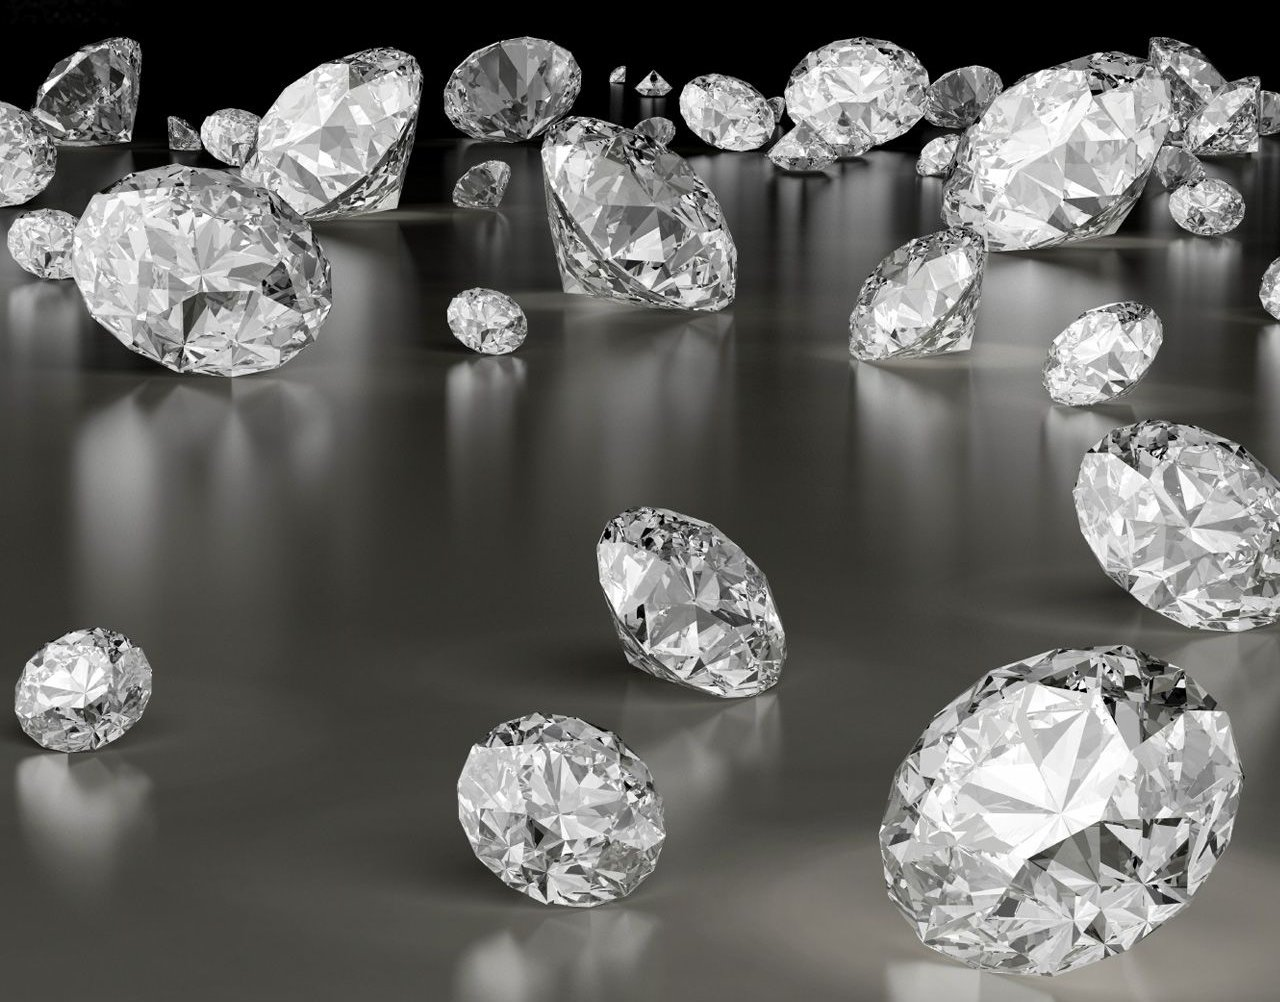
\includegraphics[width=1.13\paperwidth]{bkg}};
	\end{tikzpicture}
	
	\begin{minipage}[.2\textheight]{.4\textwidth}
    \ETHlogo[4cm]
	\end{minipage}\hfill
	\begin{minipage}[.2\textheight]{.4\textwidth}
    \begin{figure}[t]\flushright
      
\includegraphics[height=.9cm]{Logo_IPA_pos}
    \end{figure}
	\end{minipage}\vspace*{20pt}
	
	\begin{minipage}[.5\textheight]{\textwidth}
    \fig{.5}{\inserttitlegraphic}
	\end{minipage}
	
	\begin{block}{}
		\centering
		\vspace*{1pt}
		\usebeamerfont{title}\usebeamercolor[fg]{title}\textbf{\inserttitle}\\\vspace*{5pt}
		\usebeamerfont{subtitle}\insertsubtitle\\\vspace*{1pt}
	\end{block}
	\vspace*{10pt}
	\centering
	\color{black}
	\usebeamerfont{author}\textbf{\insertauthor}\par\vspace*{5pt}
	\usebeamerfont{date}\insertdate\par
}

%% FOOTLINE
\setbeamertemplate{footline}
{
  \leavevmode%
  \hbox{%
  \begin{beamercolorbox}[wd=.3\paperwidth,ht=2.25ex,dp=1ex,center]{author in head/foot}%
    \usebeamerfont{author in head/foot}\insertshortauthor\hspace*{2pt}
    (
\includegraphics[height=3.5pt]{ETHLogoWhite})
  \end{beamercolorbox}%
  \begin{beamercolorbox}[wd=.4\paperwidth,ht=2.25ex,dp=1ex,center]{title in head/foot}%
    \usebeamerfont{title in head/foot}\insertshorttitle
  \end{beamercolorbox}%
  \begin{beamercolorbox}[wd=.3\paperwidth,ht=2.25ex,dp=1ex,right]{date in head/foot}%
    \usebeamerfont{date in head/foot}\insertdate\hspace*{3em}
    \insertframenumber{} / \inserttotalframenumber\hspace*{1ex}
  \end{beamercolorbox}}%
  \vskip0pt%
}

%% HEADLINE
\setbeamertemplate{headline}
{%
  \leavevmode%
  \begin{beamercolorbox}[wd=.5\paperwidth,ht=3ex,dp=1.5ex]{section in head/foot}%
    \hbox to .5\paperwidth{\hfil\insertsectionhead\hspace*{5pt}}
  \end{beamercolorbox}%
  \begin{beamercolorbox}[wd=.5\paperwidth,ht=3ex,dp=1.5ex]{subsection in head/foot}%
    \hbox to .5\paperwidth{\hspace*{5pt}\insertsubsectionhead\hfil}
  \end{beamercolorbox}%
  \vspace*{1pt}
}
 
%% SECTION PAGE
\setbeamertemplate{section page}
{
    \begin{centering}
		\usebeamerfont{title}Section \insertsectionnumber\\\vspace*{.7cm}
		\begin{beamerboxesrounded}[shadow=true, lower=frametitle]{}
			\centering
			\vspace*{3pt}
			\usebeamerfont{frametitle}\textbf{\insertsection}\par
			\vspace*{3pt}
		\end{beamerboxesrounded}
    \end{centering}
}


\title[BCM' at PSI]{Single and Double Channel Measurements of the BCM' at PSI}
\subtitle{RD42 Meeting, Ljubljana}
\titlegraphic{Setup}
% END PREAMBEL

\begin{document}

{\setbeamertemplate{headline}{}
\setbeamertemplate{footline}{}
\maketitle}

% ======= TABLE OF CONTENTS ============
{\setbeamertemplate{headline}{}
\begin{frame}{Table of Contents}%[allowframebreaks]
	\tableofcontents[hideallsubsections]   % [pausesections]
\end{frame}}


\section{Introduction}
\subsection{Introduction}
%%%%%%%%%%%%%%%%%%%%%%%%%%%%%%%%%%%%%% FRAME 0 %%%%%%%%%%%%%%%%%%%%%%%%%%%%%%%%%%%%%%%%%%%%%%%%
\begin{frame}{Introduction}

	\begin{itemize}\itemfill
		\item after troubles at CERN also measured BCM' at PSI
		\begin{itemize}
			\item high particle rate
			\item much lower spatial resolution of the telescope
		\end{itemize}\hfill
		\item measured two diamonds with different readout boxes:
	\end{itemize}

	\begin{table}\centering\alternatecolors
		\begin{tabular}{rcc}\rowcolor{darkgray!50}\noalign{\hrule height 1.3pt}
											& \textbf{??}										& \textbf{II6-H8}								\\
			manufacturer 		& II-VI Inc.										& II-VI Inc.										\\
			diamond type 		& poly-crystal									& poly-crystal									\\
			size						& \SI{\sim4x4}{\milli\meter}		& \SI{\sim4x4}{\milli\meter}		\\
			thickness				& \SI{\sim500}{\micro\meter}		& \SI{\sim500}{\micro\meter}		\\
			amplifier				& new OSU fast Amp							& new OSU fast Amp							\\
			readout box			& \bad{1}												& \bad{2}												\\\noalign{\hrule height 1.3pt}
% 				 	& 			& 			\\
		\end{tabular}
	\end{table}
	
	\begin{itemize}\itemfill
		\item maximum 1 out of 4 amplifier channels per chip can be read out at once
		\item box 1: original box that blew up the electronics at CERN
		\begin{itemize}
			\item internal LV distribution
			\item maximum HV of \SI{300}{\volt}
		\end{itemize}
		\item box 2: different casing with all LV components of box 1 but different HV connector
	\end{itemize}

	
\end{frame}

\subsection{Measurements}
%%%%%%%%%%%%%%%%%%%%%%%%%%%%%%%%%%%%%% FRAME 1 %%%%%%%%%%%%%%%%%%%%%%%%%%%%%%%%%%%%%%%%%%%%%%%%
\begin{frame}{Measurements}

	\begin{itemize}\itemfill
		\item avoid noise from programming pc:
		\item lock programming into the amps before every change of channel or chip configuration
		\begin{itemize}
			\item connect \SI{500}{\milli\volt} supply voltage 
			\item hook up DB connector to the readout boxes
			\item program chip 
			\item disconnect DB
			\item ground supply voltage line
		\end{itemize}
	\item every data run is preceded by a pumping run at high rate of the same duration
	\end{itemize}


	\begin{table}\centering\alternatecolors
		\begin{tabular}{ccccc}\rowcolor{darkgray!20}\noalign{\hrule height 1.3pt}
			\textbf{Box}	& \textbf{Chip}	& \textbf{Channel}	& \textbf{Bias [V]}	& \textbf{Events [M]}	\\ 
			1							&	1				 			& 1									&	\SI{\pm200}{}			& 0.8\\
			1							&	1				 			& 1									&	\SI{\pm300}{}			& 0.8\\
			1							&	2			 				& 1									&	\SI{\pm200}{}			& 0.8\\
			1							&	2				 			& 1									&	\SI{\pm300}{}			& 0.8\\
			1							&	1 \& 2	 			& 1									&	\SI{\pm200}{}			& 0.8\\\hline
			2							&	1 \& 2	 			& 1									&	\SI{\pm500}{}			& 1.6\\
			2							&	1 \& 2	 			& 1									&	\SI{\pm1000}{}		& 1.6\\\noalign{\hrule height 1.3pt}
		\end{tabular}
	\end{table}
	
\end{frame}

\section{Test Site}
%%%%%%%%%%%%%%%%%%%%%%%% FRAME 0 %%%%%%%%%%%%%%%%%%%%%%%%%%%%%%%
{
	\setbeamertemplate{footline}{}
	\begin{frame}
		\begin{tikzpicture}[remember picture,overlay]
			\node[at=(current page.center)] {
				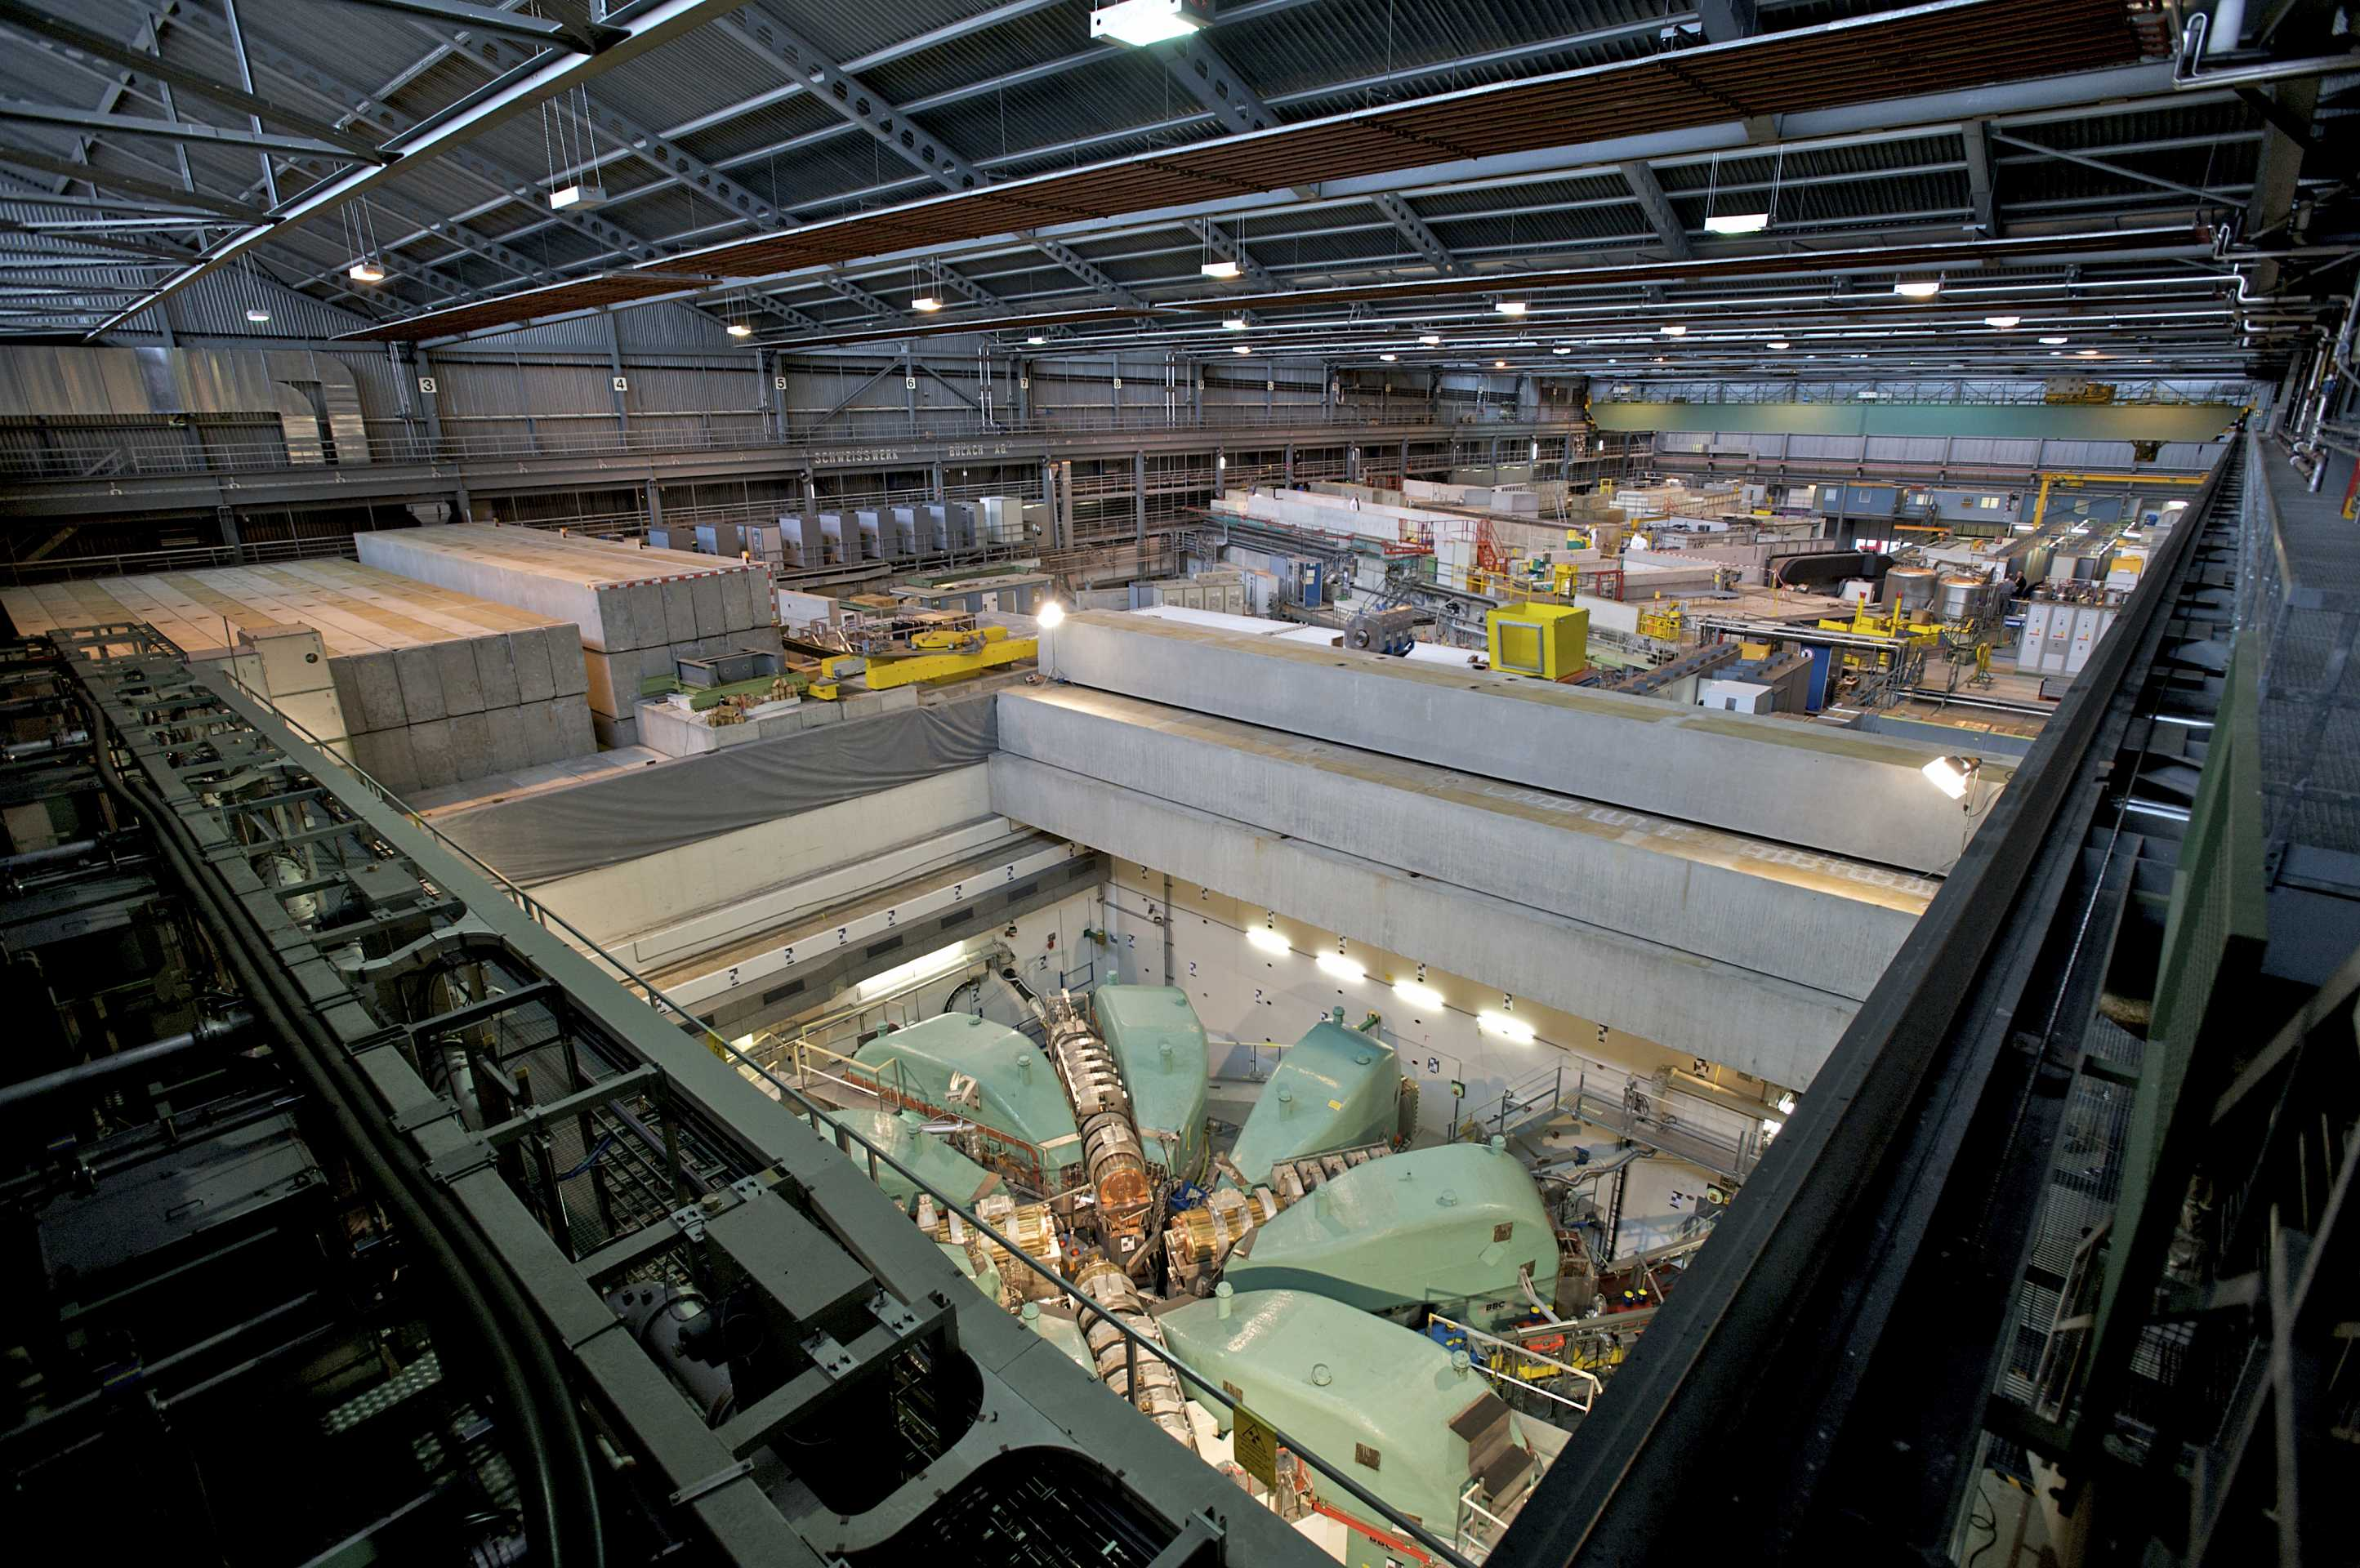
\includegraphics[width=1.15\paperwidth]{Cyclo2}};
		\end{tikzpicture}
		
	\end{frame}
}
%%%%%%%%%%%%%%%%%%%%%%%% FRAME 1 %%%%%%%%%%%%%%%%%%%%%%%%%%%%%%%
\begin{frame}{Test Site}

	\begin{itemize}
		\itemfill
		\item High Intensity Proton Accelerator (HIPA) at PSI \ra beam line PiM1
		\item clean positive pion beam (\SI{\sim98}{\%} $\uppi^+$) with momentum of \SI{260}{\mega\electronvolt\per c} 
		\begin{itemize}
			\item \SI{75}{\%} of the signal size at CERN! (\SI{120}{\giga\electronvolt\per c})
		\end{itemize}
% 		\item \good{tunable particle fluxes from \orderof{\SI{1}{\kilo\hertz\per cm^2}} to \orderof{\SI{10}{\mega\hertz\per cm^2}}}
		\item \bad{significant multiple scattering \ra worsens resolution}
	\end{itemize}
	
	\subfigs[\subfig[.36]{.48}{Cyclo1}]{\subfig[.3]{.5}{Cyclo3}}{\subfig[.22]{.25}{Target}}\vspace*{-10pt}

\end{frame}

\section{Results}
\subsection{Leakage Currents}
%%%%%%%%%%%%%%%%%%%%%%%%%%%%%%%%%%%%%% FRAME 0 %%%%%%%%%%%%%%%%%%%%%%%%%%%%%%%%%%%%%%%%%%%%%%%%
\begin{frame}{Box 1}

	\begin{itemize}\itemfill
		\item all pads/channels of the two amplifier chips are connected to the same HV line
		\item pumping at higher rate induces leakage current in the sensor
	\end{itemize}\vspace*{-10pt}
	
	\only<1>{\fig[r]{.45}{LC200}[Box 1 at \SI[retain-explicit-plus]{+200}{\volt}]}
	\only<2>{\fig[r]{.45}{LC300}[Box 1 at \SI[retain-explicit-plus]{+300}{\volt}]}\vspace*{-10pt}
	
	\begin{itemize}
		\item<1-> stable behaviour at \SI[retain-explicit-plus]{+200}{\volt}
		\item<2> erratic currents up to \orderof{\SI{2}{\micro\ampere}} at high rates at \SI[retain-explicit-plus]{+300}{\volt}
	\end{itemize}
	
\end{frame}
%%%%%%%%%%%%%%%%%%%%%%%%%%%%%%%%%%%%%% FRAME 1 %%%%%%%%%%%%%%%%%%%%%%%%%%%%%%%%%%%%%%%%%%%%%%%%
\begin{frame}{Box 2}
	
	\only<1>{\fig[r]{.45}{LCB2P}[Box 2 at positive voltage]}
	\only<2->{\fig[r]{.45}{LCB2N}[Box 2 at negative voltage]}
	
	\begin{itemize}\itemfill
		\item<1-> very stable behaviour up to \SI{\pm1}{\kilo\volt}
		\item<1-> slight increase at \SI[retain-explicit-plus]{+1}{\kilo\volt}
		\item<2-> exponential increase at \SI{-1}{\kilo\volt}
		\item<3-> current positive independed of bias ...
	\end{itemize}
	
\end{frame}

\subsection{Waveforms}
%%%%%%%%%%%%%%%%%%%%%%%%%%%%%%%%%%%%%% FRAME 2 %%%%%%%%%%%%%%%%%%%%%%%%%%%%%%%%%%%%%%%%%%%%%%%%
\begin{frame}{Positive Bias}

	\begin{itemize}\itemfill
		\item all signal polarities are opposite of the bias 
		\item pumping at higher rate induces leakage current in the sensor
	\end{itemize}\vspace*{-10pt}
	
	\only<1>{\fig[r]{.4}{WF200-0}[Single waveform 0 \SI[retain-explicit-plus]{+200}{\volt}]}
	\only<2>{\fig[r]{.4}{WF200-1}[Single waveform 1 \SI[retain-explicit-plus]{+200}{\volt}]}
	\only<3>{\fig[r]{.4}{WF200-2}[Single waveform 2 \SI[retain-explicit-plus]{+200}{\volt}]}
	\only<4>{\fig[r]{.4}{WF200-3}[Single waveform 3 \SI[retain-explicit-plus]{+200}{\volt}]}
	\only<5>{\fig[r]{.4}{WF200-4}[Single waveform 4 \SI[retain-explicit-plus]{+200}{\volt}]}
	\only<6>{\fig[r]{.4}{WF200-5}[Single waveform 5 \SI[retain-explicit-plus]{+200}{\volt}]}
	\only<7>{\fig[r]{.4}{WF200-6}[Single waveform 6 \SI[retain-explicit-plus]{+200}{\volt}]}
	
	\begin{itemize}
		\item pulses usually have a flattish top and probably don't reach the maximum
	\end{itemize}
	
\end{frame}

\section{Conclusion}
\begin{frame}{Conclusion}

	\begin{minipage}[c][.6\textheight]{\textwidth}
		\begin{itemize}\itemfill
			\item successfully measured two BCM' modules at PSI
			\item only channel 1 of each chip working at low noise
			\item possible to read out two channels of independent chips at the same time
			\item SNR at \SI{1}{\kilo\volt}:
			\item shape of negative signals becomes flat before reaching the highest point
			\item rise time at positive voltage: 
			\item coupling between connected and non-connected channels
		\end{itemize}
	\end{minipage}
	
\end{frame}

\setbeamertemplate{footline}{}
\begin{frame}

	\begin{tikzpicture}[remember picture,overlay]
		\node[at=(current page.center)] {
			
\includegraphics[width=1.13\paperwidth]{delfin}};
	\end{tikzpicture}
	
\end{frame}
  % FINAL PAGE

\end{document} % DOCUMENT END

